\chapter{Mobilidade em São Paulo}
\label{cap:mobilidade-rmsp}

Para fornecer uma melhor compreensão do cenário de nossa análise, esta seção
descreve as características da Região Metropolitana de S\~ao Paulo (RMSP) e os dados da
última pesquisa OD realizada na região. Para evitar antagonismos entre a
Região Metropolitana de S\~ao Paulo Área e a cidade de S\~ao Paulo, vamos nos
referir à cidade como capital ou simplesmente S\~ao Paulo e vamos nos referir à
área metropolitana como RMSP ou simplesmente área metropolitana. 

\section{Região Metropolitana de São Paulo}

O estado de S\~ao Paulo está localizado no litoral sudeste do Brasil. A Regi\~ao
Metropolitana de S\~ao Paulo é a região mais populosa da América do Sul. De acordo
com o Instituto Brasileiro de Geografia e Estatística \citep{ibge2020}, a RMSP contabilizou $21,9$
milhões de cidadãos em 2020, o que representa cerca de 10\% da população
brasileira. A RMSP é composta por 39 municípios em uma área de \num{7946.84} $km^{2}$. A
cidade de São Paulo é a capital do estado de São Paulo e está localizada no
centro da região metropolitana. A Figura \ref{fig:map-spma} mostra os 39 municípios que compõem a
RMSP. A capital é a cidade mais populosa do Brasil, com 12.3 milhões de
habitantes. Na RMSP, as outras cidades com mais habitantes são Guarulhos (1.4
milhão), São Bernardo do Campo (844 mil), Santo André (721 mil) e Osasco (699
mil).

\begin{figure}[!htb]
  \centering
  \captionsetup{justification=centering}
  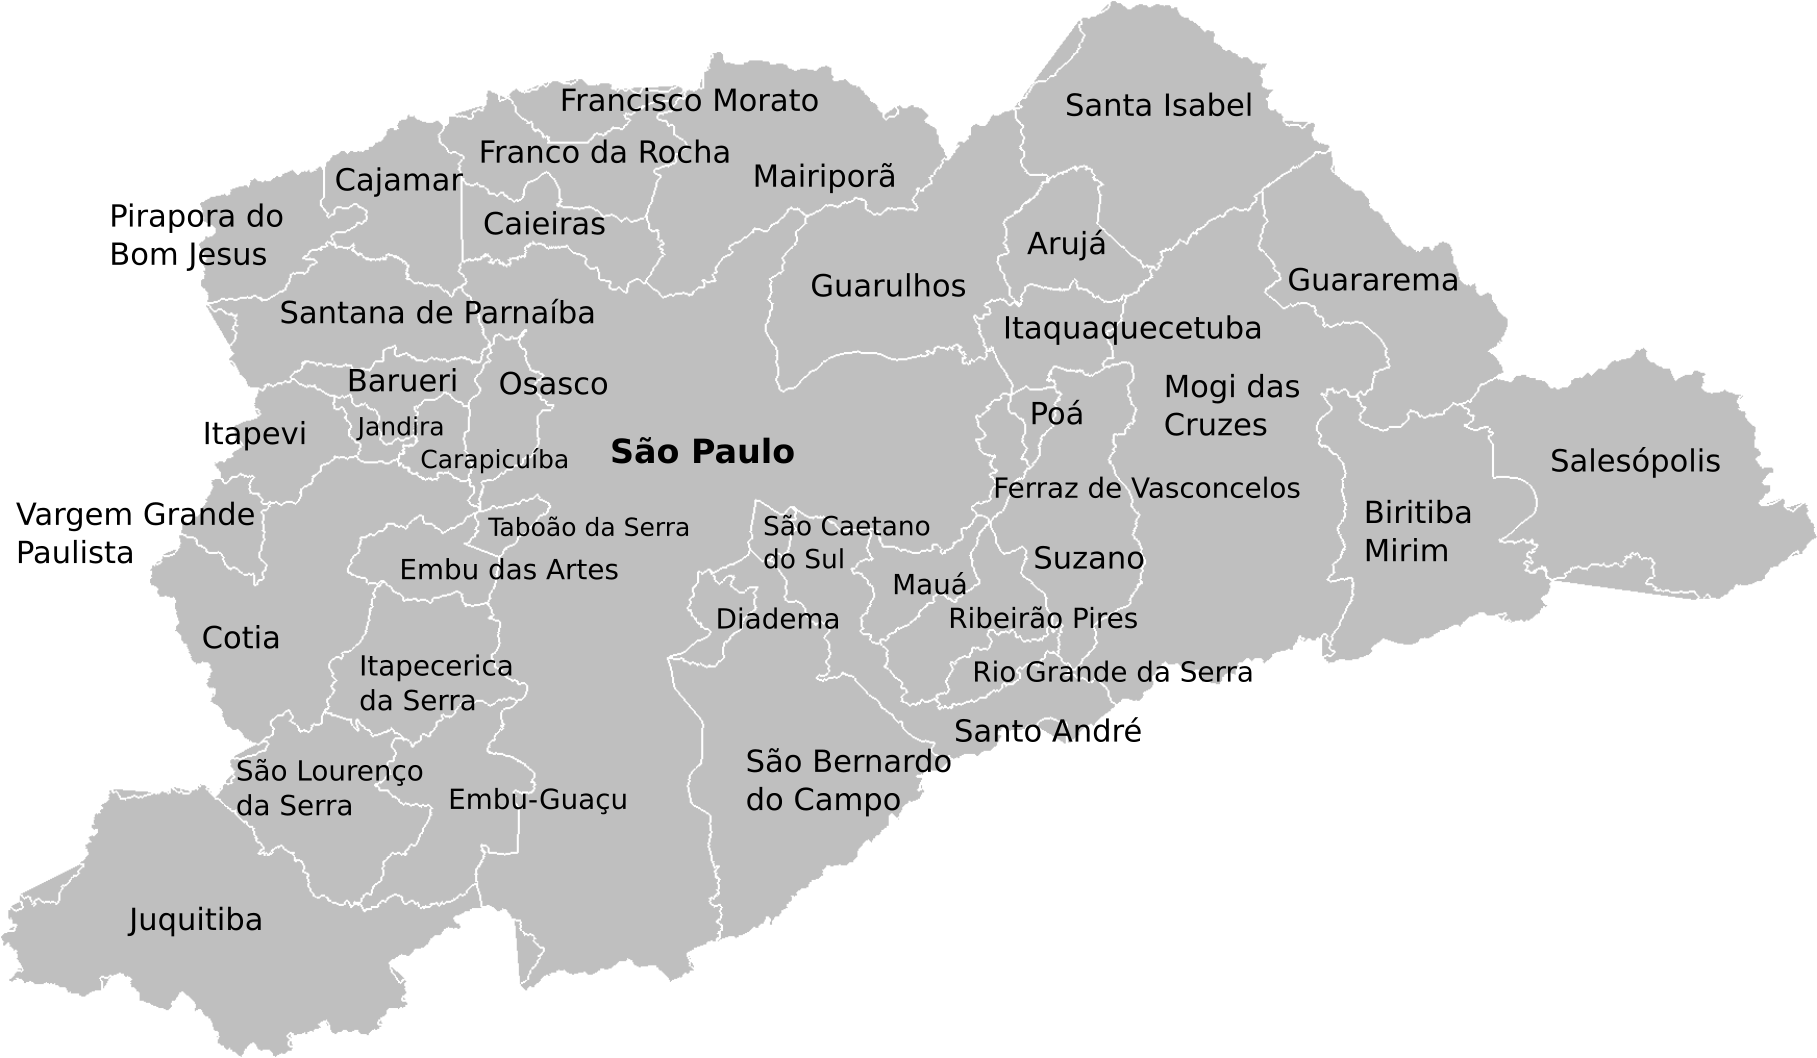
\includegraphics[width=0.95\textwidth]{../figuras/map-spma.png}
    \caption{Municípios da RMSP.\label{fig:map-spma}}
\end{figure}

A capital e as cidades mais próximas concentram a maior parte das oportunidades
de emprego, instalações e serviços públicos, universidades, museus e opções
de entretenimento. Portanto, há um grande deslocamento diário para o centro da
capital e seus arredores. Em São Paulo, os bairros próximos ao centro da
cidade são mais valorizados, portanto, morar nessas partes da cidade tem um maior custo.
Pessoas com menos condições financeiras costumam residir na periferia da capital
ou em outras cidades da RMSP, por isso, algumas cidades da RMSP tornaram-se cidades
dormitório para aqueles que não podem pagar comprar ou alugar uma casa na
capital.

Em relação à infraestrutura de transporte, a capital possui uma rede metroviária
que atende as regiões norte, sul, leste, oeste, sudoeste e sudeste da cidade.
Existem algumas linhas de metrô, a maioria delas cruzando o centro da capital, o
que limita o acesso ao sistema de metrô a algumas regiões da cidade. As demais
cidades não possuem sistemas de metrô, mas existe um outro sistema ferroviário
metropolitano que atende várias cidades do entorno e que é integrado ao sistema
metroviário da capital.

Cada cidade tem seu próprio sistema de ônibus e há um sistema de ônibus
intermunicipal para ligar cidades vizinhas. Durante o século 20, até o final da
década de 1990, a maioria dos investimentos no transporte foram guiados por uma
abordagem focada no transporte individual de carros em detrimento do transporte
público \citep{rolnik2011}. Os objetivos eram ampliar estradas e ruas para
atender à crescente demanda por carros particulares. Nas últimas duas décadas,
os governos locais têm investido mais em políticas de incentivo ao transporte
público, como implantação de corredores de ônibus e substituição da frota de
ônibus, construção de novas linhas de metrô e modernização do sistema
ferroviário. Além disso, há uma crescente infraestrutura de ciclismo na capital
que vem sendo expandida na última década. Embora esses investimentos tenham
aumentado nos últimos anos, a RMSP ainda sofre com o congestionamento do
tráfego, principalmente nos horários de pico \citep{rolnik2011,ricardo:18}.
Assim, é necessário um melhor entendimento do o comportamento do trânsito na
RMSP para propor novas políticas de melhoria da mobilidade para seus cidadãos.



\section{Pesquisa Origem-Destino}
\label{sec:pesquisa-od}

A pesquisa Origem-Destino (OD) é a principal fonte de informações de mobilidade
sobre a RMSP. Ela é realizada pela Companhia Metropolitana de São Paulo (Metrô)
a cada dez anos, tendo a primeira aplicação em 1967. A última pesquisa OD de
2017 (OD17) tem informações sobre \num{157992} viagens de pessoas registradas
aleatoriamente na RMSP. Cada viagem possui um fator de expansão associado, que é
a extrapolação estatística para o tamanho da população que cada viagem
representa. O fator de expansão somado de todas as entradas da pesquisa resulta
no total de 42 milhões de viagens em um dia útil típico. Os dados representam
uma ampla amostragem da população total e possuem resultados sólidos com uma
pequena margem de erro de 6\% e intervalo de confiança de 92\%
\citep[p.18]{odmanual:17}. As viagens ocorrem por diferentes motivos, como
trabalho, casa, estudo e lazer e diferentes modos de viagem, como caminhada,
carro, metrô e trem. A Figura~\ref{fig:reason_mode} mostra a distribuição das
viagens por meio de transporte e por motivação e a
Figura~\ref{fig:trips_by_hour} mostra a distribuição das viagens pelas horas do
dia. Os gráficos foram construidos a partir dos dados extraídos da OD17
aplicando-se o fator de expansão de cada viagem.

\begin{figure}[ht]
\captionsetup[subfigure]{justification=centering}
\subcaptionbox{Modo de transporte\label{fig:travel-mode}}[0.49\linewidth][l]{%
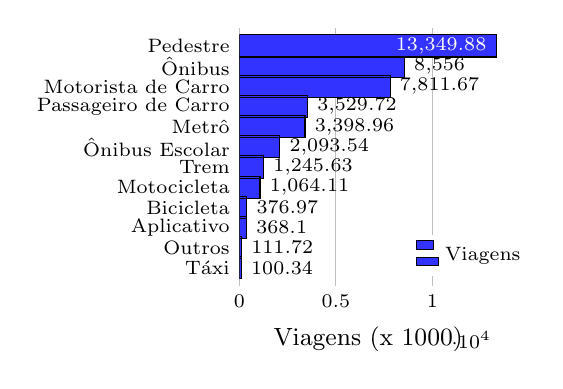
\begin{tikzpicture}
  \begin{axis}[
    width=.4\columnwidth,
    height=11.5\baselineskip,
    xbar=0pt,
    bar width=8pt,
    bar shift = 0pt,
%    ytick = data,
    y axis line style = { opacity = 0 },
    tickwidth         = 0pt,
    enlarge y limits  = 0.08,
    enlarge x limits  = 0,
    symbolic y coords = {Táxi,Outros,Aplicativo,Bicicleta,Motocicleta,Trem,Ônibus Escolar,Metrô,Passageiro de Carro,Motorista de Carro,Ônibus,Pedestre},
    ytick distance=1,
    xlabel near ticks,
    xlabel={Viagens (x 1000)},
    xmin=0,
    xmajorgrids,
    label style={font=\small},
    tick label style={font=\scriptsize},
    nodes near coords,
    every node near coord/.append style={font=\scriptsize,color=black},
    legend style={at={(0.9,0.2)},anchor=north,legend columns=-1,font=\scriptsize,draw=none},
  ]
  \addplot[fill=blue!80] coordinates {(100.34,Táxi)(111.72,Outros)(368.10,Aplicativo)(376.97,Bicicleta)(1064.11,Motocicleta)(1245.63,Trem)(2093.54,Ônibus Escolar)(3398.96,Metrô)(3529.72,Passageiro de Carro)(7811.67,Motorista de Carro)(8556,Ônibus)};
  \addplot[fill=blue!80, every node near coord/.append style={xshift=-4em,font=\scriptsize,color=white},] coordinates {(13349.88,Pedestre)};
    \legend{Viagens}
  \end{axis}
\end{tikzpicture}
}%
\subcaptionbox{Motivo da viagem\label{fig:travel-reason}}[0.49\linewidth][r]{%
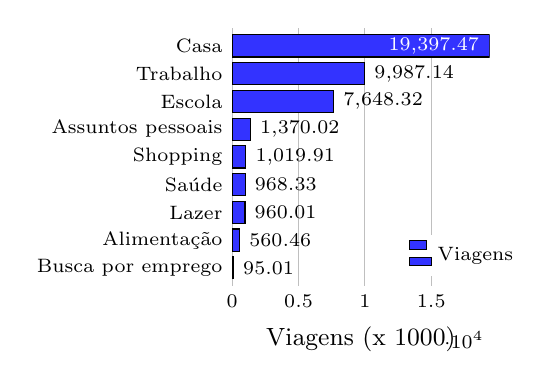
\begin{tikzpicture}
  \begin{axis}[
    width=.4\columnwidth,
    height=11.5\baselineskip,
    xbar=0pt,
    bar width=8pt,
    bar shift = 0pt,
%    ytick = data,
    y axis line style = { opacity = 0 },
    tickwidth         = 0pt,
    enlarge y limits  = 0.08,
    enlarge x limits  = 0,
    symbolic y coords = {Busca por emprego,Alimentação,Lazer,Saúde,Shopping,Assuntos pessoais,Escola,Trabalho,Casa},
    ytick distance=1,
    xlabel near ticks,
    xlabel={Viagens (x 1000)},
    xmin=0,
    xmajorgrids,
    label style={font=\small},
    tick label style={font=\scriptsize},
    nodes near coords,
    every node near coord/.append style={font=\scriptsize,color=black},
    legend style={at={(0.9,0.2)},anchor=north,legend columns=-1,font=\scriptsize,draw=none},
  ]
  \addplot[fill=blue!80] coordinates {(95.01,Busca por emprego)(560.46,Alimentação)(960.01,Lazer)(968.33,Saúde)(1019.91,Shopping)(1370.02,Assuntos pessoais)(7648.32,Escola)(9987.14,Trabalho)};
  \addplot[fill=blue!80, every node near coord/.append style={xshift=-4em,font=\scriptsize,color=white},] coordinates {(19397.47,Casa)};
  \legend{Viagens}
  \end{axis}
\end{tikzpicture}
}%
\caption{Registros por modo de transporte e por motivo da viagem.}
\label{fig:reason_mode}
\end{figure}

\begin{figure}
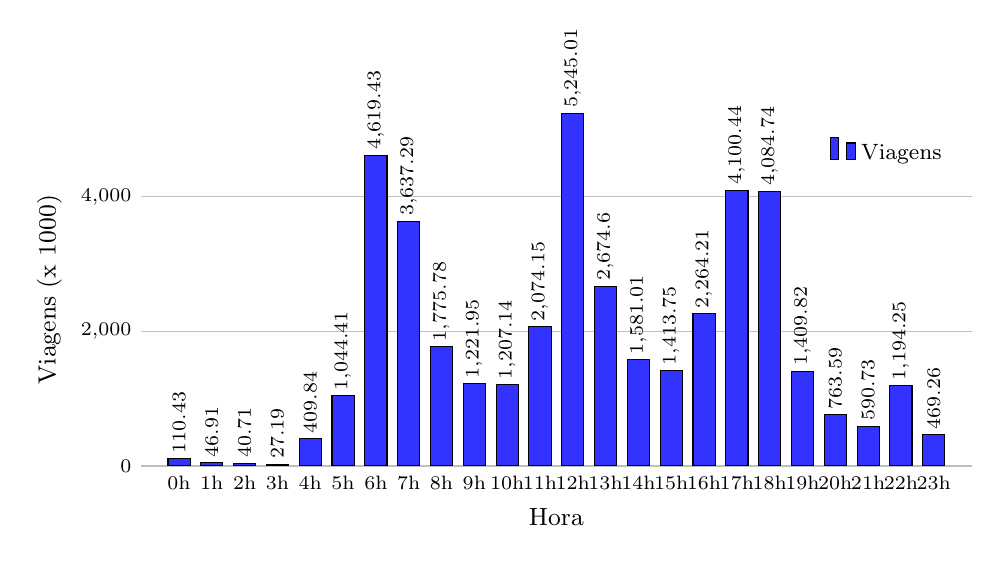
\begin{tikzpicture}
  \begin{axis}[
    ybar=0pt,
    bar width=8pt,
    bar shift = 0pt,
    width=\textwidth,
    height=0.5\textwidth,
    tickwidth         = 0pt,
    enlarge y limits  = 0,
    enlarge x limits  = 0.05,
    symbolic x coords = {0h,1h,2h,3h,4h,5h,6h,7h,8h,9h,10h,11h,12h,13h,14h,15h,16h,17h,18h,19h,20h,21h,22h,23h},
    xtick = data,
    ylabel near ticks,
    ylabel={Viagens (x 1000)},
    xlabel={Hora},
    ymin=0,
    ymajorgrids,
    y axis line style = { opacity = 0 },
    label style={font=\small},
    tick label style={font=\scriptsize},
    nodes near coords,
    every node near coord/.append style={font=\scriptsize,color=black,yshift=0.05cm,rotate=90,anchor=west,inner sep=0.3pt},
    legend style={at={(0.9,0.95)},anchor=north,legend columns=-1,font=\footnotesize,draw=none},
  ]
  \addplot[fill=blue!80] coordinates {(0h,110.43)(1h,46.91)(2h,40.71)(3h,27.19)(4h,409.84)(5h,1044.41)(6h,4619.43)(7h,3637.29)(8h,1775.78)(9h,1221.95)(10h,1207.14)(11h,2074.15)(12h,5245.01)(13h,2674.60)(14h,1581.01)(15h,1413.75)(16h,2264.21)(17h,4100.44)(18h,4084.74)(19h,1409.82)(20h,763.59)(21h,590.73)(22h,1194.25)(23h,469.26)};
  \legend{Viagens}
  \end{axis}
\end{tikzpicture}
\caption{Viagens por hora do dia.}
\label{fig:trips_by_hour}
\end{figure}

Como mostra a Figura~\ref{fig:reason_mode}, a maioria das viagens na cidade são feitas por
pedestres. Normalmente, viagens de pedestres cobrem pequenas distâncias (624m em média)
e ficam dentro de um único distrito da cidade. Podemos perceber também que há
um número significativo de viagens de carro e de transporte público
(ônibus, metrô e trem), a maioria mais longa (7,7 km em média), principalmente
de trem e metrô (13,5 km em média). Olhando para viagens por hora (Figura~\ref{fig:trips_by_hour}),
é possível notar que o trânsito na RMSP tem três picos principais: pela manhã (6h às 8h),
na hora do almoço (meio-dia) e no início da noite (17h às 19h).

Os \num{157992} registros da pesquisa OD possuem inúmeros atributos sobre as
viagens. Os mais relevantes para nosso estudo, no entanto, são as coordenadas de
origem e destino e o fator de expansão da viagem. Outros atributos são o horário
de saída, o meio de transporte (17 categorias: trem, metrô, motorista
de carro, passageiro de carro, ônibus da cidade de São Paulo e de outras
cidades, ônibus intermunicipal, monotrilho, veículo fretado, ônibus escolar,
táxi regular, táxi não regular, motorista de motociclista, passageiro de
motociclista, pedestre, bicicleta e outros) e o motivo da viagem (9 categorias:
casa, trabalho, estudo, assuntos pessoais, compras, saúde, lazer, alimentação e
busca por emprego).

A Figura~\ref{fig:cluttered-graph} mostra as viagens da pesquisa OD desenhadas sobre o mapa do
RMSP, onde cada linha representa uma trajetória da OD. A extrema oclusão na figura
impede a visualização de trajetórias individuais, padrões de tráfego ou conexões
entre as regiões do mapa. A partir dessa imagem, podemos apenas inferir a
existência de tráfego intenso na maior parte da região metropolitana e uma
concentração significativa desse tráfego no centro de São Paulo. Além disso,
esta imagem não mostra nenhum dos atributos de dados disponíveis, exceto O e D.
Portanto, as técnicas de filtragem e agregação são essenciais para simplificar a
visualização e torná-la compreensível.

\begin{figure}[!htb]
  \centering
  \captionsetup{justification=centering}
  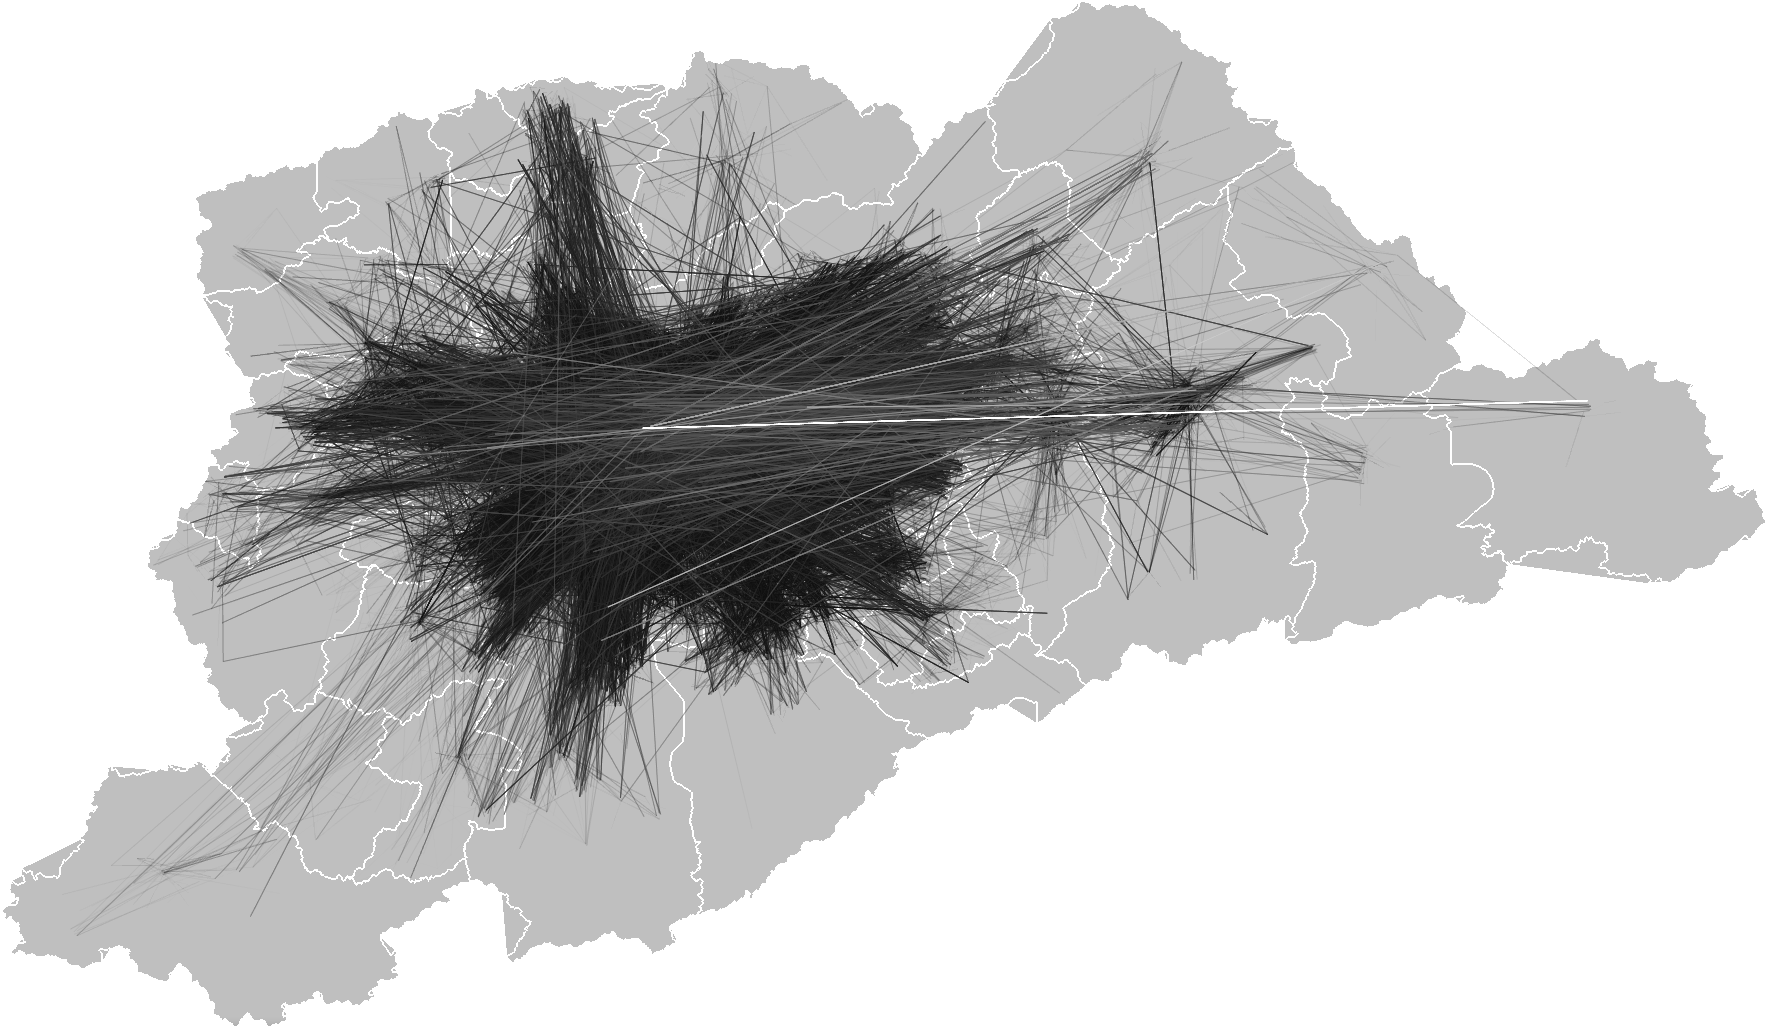
\includegraphics[width=0.95\textwidth]{figuras/unbundled-edges+grayscale+512px.png}
  \caption{Viagens da OD sobre a RMSP. As linhas ligam os pontos de origem e destino. \label{fig:cluttered-graph}}
\end{figure}
